\chapter{Introduction}
\section{Optical Tweezers}
Precise manipulation of micro-particles and measurements of 
microscopic forces has been development in scientific research.
It has long been known that the motion of microscopic particles 
is due to multiple random collisions, measuring the average 
momentum transferred is often done by generating a potential 
well constructed using light - more commonly referred to as 
optical tweezing. 

Since the mid 1900's it was known that light can transfer momentum 
to a medium, being referred to as 'radiation pressure', initially 
this was applied by transferring both linear and angular momentum 
to suspended mirrors \cite{Beth1936MechanicalDA}. This allowed 
researchers to measure the momentum of light carried by a single 
photon \cite{Beth1936MechanicalDA}. It was Ashkin who showed that 
by constructing a precise wavefront one could confine biological 
cells as small as a few microns \cite{Ashkin1970}. This was 
especially useful as the process was non-invasive, preserving the 
internal organelles while keeping the cell trapped. 

The working principle is that a collimated light source - such as 
a laser - can confine a particle in the plane perpendicular to the 
beam \cite{Ashkin1970}. The radiation pressure previously observed 
is due to the momentum transferred to the target, when directed at 
an isotropic scatterer the light the momentum transfer is minimised
when the target particle is centred on the laser beam. Initially, 
confinement in the direction of the laser was achieved by matching 
the laser power so that the radiation pressure transferred would equal 
the mass of the target \cite{Ashkin1970}. Soon after, Ashkin showed 
that the by focusing the light source through a lens would confine 
the target particle in all 3 Cartesian directions regardless of the
laser power \cite{Ashkin1980}. The use of lenses to create a focal
point allowed for the development of much stronger optical traps that
could trap complex particles and biological materials. 

Beyond simply observations, optical tweezing allowed for precise 
measurements of microscopic forces. Later it would be used to probe microscopic properties such as the Brownian forces exerted within a 
pure vacuum \cite{Ahn2018, Monteiro2018}. Due to the predictable 
behaviour of light, optical tweezers have become essential for 
measuring and exerting precise forces on the magnitude of pico-newtons.
However, these measurements are based on the idea that the trapped 
particle in question is an isotropic scatterer, meaning that particle 
is can be approximated as a sphere. This is an apt approximation if 
we only care about measuring the force exerted due to translational 
motion. In reality, rotational motion is a significant factor to the 
trajectory of non-spherical particles, in which case our understanding
of how light interacts with particles is incomplete without considering
the optical torque exerted by a focused beam.

\subsection{Optical Torque and rotation}
\label{sec:opt_torque}
Electromagnetic fields can transfer both linear and angular momentum \cite{Beth1936MechanicalDA}; more accurately the field is said to have 
both orbital and spin momentum. Though there is some debate on how to decompose the total momentum into these two components \cite{Bruce2020, Svak2018}, for this project we do not need to calculate the exact 
quantities and will instead look at the broader effects of both 
components. Orbital angular momentum arises from the shape of the 
wavefront of the particular field in question; for simple Gaussian 
beams the wavefronts are uniform and equally spaced resulting in the 
typical radiation pressure that Ashkin and co demonstrated 
\cite{Ashkin1980}. However, higher order modes of a Gaussian beam (for example: Laguerre-Gaussian modes) have non-uniform wave fronts meaning 
the orbital momentum has both angular and linear components; depending 
on the relative size of the target particle one can induce rotation, 
or orbiting \cite{Bruce2020, Courtial2000}. 

Spin angular momentum (SAM) is attributed to the spin density of 
the field, early research has shown that the spin density is non-
zero for any beam despite the fact that the total SAM transferred 
to a medium is 0 \cite{Svak2018, Bliokh2014}. This has sparked 
debate if SAM is even a physical quantity as it does not aid in 
the transport of energy directly \cite{Bliokh2014} and so cannot 
be directly observed in some cases despite being non-zero. This 
paradox is resolved by representing the wave as an array of spin 
momentum loops that cancel one-another out when the medium is 
homogeneous.Spacial inhomogeneities cause these spin loops to no 
longer be equal, resulting in non-zero spin density, anisotropic 
mediums (such as birefringent crystal lattices) experience a 
transfer of spin angular momentum, imparting an optical torque.

Birefringence is a material property often seen in crystalline 
materials, where the crystal lattice has a different structure 
dependent on its orientation. Since light is composed of waves 
that propagate in orthogonally to one another, a birefringent 
material will refract light differently depending on the light's 
polarisation. Therefore it can be said that the material has 
two separate refractive indices. For circularly polarised light 
this inhomogeneity results in a high degree of SAM being 
transferred to the target object \cite{Parkin2009, Arita2016}. 
The greater the difference between the two refractive indices the 
greater the angular momentum transfer.

The ability to transfer angular momentum has been exploited 
to rotate microspheres as fast as 1000 Hz while suspended 
in a bulk medium \cite{Arita2016} as well as a means of 
measuring the local temperature and shear response of said 
medium \cite{Millen2014, RodriguezSevilla2018}. Calculating 
the optical torque applied to a birefringent material is given 
via:
\begin{equation}
	\label{eq:opt_torque}
	\begin{aligned}
		\tau_{opt} =& -\frac{\epsilon}{2\omega_{laser}}E_0^2sin(kd(\Delta n))cos2\theta sin2\phi 
		\\ &+  \frac{\epsilon}{2\omega_{laser}}E_0^2 (1-cos(kd(\Delta n))sin2\phi)
	\end{aligned}
\end{equation}

Where $\Delta n$ is the difference between the two refractive 
indices, $\theta$ is the angle between the particle's long 
axis and the polarisation vector of the local EM field, and 
$\phi$ is the phase shift in the EM field. The first term 
represents the 'orientational' torque which aligns the long 
axis of the particle with the electric field, when aligned 
$\theta=0$ meaning the entire term is negligible for particle's 
with a stable orientation. The second term is due purely to the 
polarisation of the laser, for circularly polarised light 
$\phi=\pi/4$ thus maximising the torque transferred to the 
target particle. Eq.~\eqref{eq:opt_torque} is only applicable 
for particles with a known birefringence, but there are other 
mechanisms that result in optical torque.

A common example is shape induced birefringence. If a particle 
has an anisotropic shape, it is more susceptible to being 
polarised along its longer axis than its shorter axis. Consider, 
for example, an ellipsoid elongated along one of its primary 
axis' ($r_z > r_x = r_y$). In a plane polarised beam such a 
particle will align with the polarisation vector. Therefore, 
the particle will rotate as angular momentum is transferred 
along its long axis. One common feature, regardless of shape,
is that a particle with shape birefringence will rotate when 
it lies perpendicular to the direction of propagation. This 
is seen most evidently with spherical dimers \cite{Ahn2018, 
Reimann2018} but even for elliptical particles rotational 
motion is only detected when their long axis is not aligned 
with the direction of propagation \cite{Zhu2021, Mihiretie2014}.

\begin{figure}[h!]
	\centering
	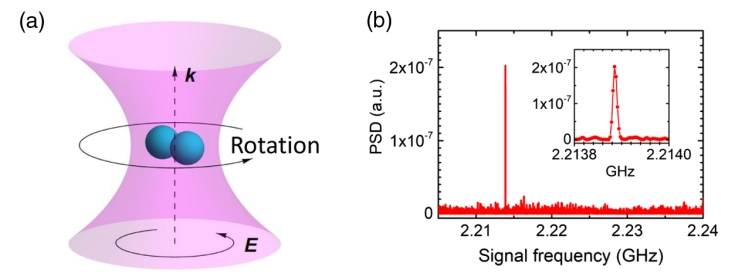
\includegraphics[width=\linewidth]{dimer_rotation.jpeg}
	\caption{Example of nano-dimer undergoing optical rotation 
		in a circularly polarised beam. Due to the dimer's 
		anisotropic susceptibility it is polarised along its 
		long axis, the dimer will therefore align its long axis 
		with the polarization vector. Reproduced with permission 
		from \cite{Reimann2018}.}
\end{figure}

Often the optical torque experienced is far greater than similar 
spherical particles that are birefringent \cite{Bruce2020}. 
Currently spherical dimers are being rotated in vacuums to 
measure quantum forces and torques \cite{Ahn2018, Reimann2018}. 
There are some alternative cases where particles are rotated 
while not being aligned in the plane of the polarisation. However 
in these cases their shape is often specifically engineered to 
scatter light in such a way that the net momentum change always
occurs in one direction regardless of the laser polarisation 
\cite{Higurashi1994}. 

Other examples of optical torque is when an anisotropic 
particle is aligned with the beam's direction of propagation 
(in which case $\theta=\pi/2$ and the first term disappears). 
This is analogous to an optically trapped sphere, where 
alongside a restoring force the particle also experiences a 
restoring torque. This seemingly random rotational motion is 
referred to as libation \cite{Bruce2020},often in typical 
suspension trapping situations (where the particle is suspended 
in a fluid) the rotational motion is washed out by the 
translational motion. As such, many experiments elect to trap 
in low pressure environments to precisely measure the optical 
torque being exerted by the optical trap \cite{Ahn2018}. This 
has lead experiments to try and achieve '0 kelvin' motion, 
where by trapping a silica dimer they were able to restrict its 
motion using 3 optical traps simultaneously. Despite this, they 
found that the dimer's rotational motion about its long axis 
could not be controlled leading to the undesired rotational
modes \cite{Bang2020}.

The detection and measurement of optical torque is still a 
field of intense research, not only does it have potential 
to understand quantum fluctuations in a particle's motion 
but also allows for the creation of more effective
micro-rotors. The latter being especially pertinent for 
understanding the behaviour of fluids experiencing localised 
shearing.

\subsection{Characterisation of rotational motion}
Rotational motion about a single axis is easiest to account for.  
When the power spectra of elliptical polystyrene particles was 
fitted by Yogesh \textit{et al} \cite{Yogesha2011PreciseCO}, they 
assumed that the rotational motion was purely in the transverse
plane. As such they did not have to account for any variance in 
the trapping strength due to orientation nor did they need to
consider non-periodic rotational behaviour. In the case where 
rotational motion is stochastic the problem is more complex. 
For example, when an optical fibre trap characterisation 
technique was implemented by Saffron \textit{et al} 
\cite{BarZiv1997, Meller1998}, they were able to use dynamic 
light scattering to characterise both the axial and lateral 
trap stiffness acting on microspheres. 

\begin{figure}[h!]
	\centering
	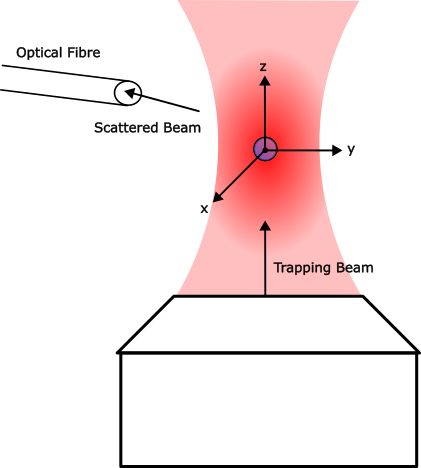
\includegraphics[width=\linewidth]{BarZivDiagram.png}
	\caption{Diagram depicting the setup used by \cite{BarZiv1997}, 
	a microsphere is trapped by a focused beam. The scattered beam
	is collected by an optical fibre situated close to the trapped
	sphere. Using DLS they are able to relate the autocorrelation 
	function of the collated signal to characterise the trap stiffness 
	of the optical trap.}
\end{figure}

The only drawback admitted to in their work was that the technique 
was constrained to isotropic scatters as their theoretical model 
for describing the auto-correlation function was predicated on the 
fact that any variations in the signal are due to the particles 
translational motion within the confines of a cylindrical trap 
\cite{BarZiv1997}. Where the upper limit of the cylindrical trap 
is given by the Rayleigh range ($z_R = n\omega_0/NA$). This is 
discussed further in chapter 3 in the discussion of dimer dynamics, 
the axial traps of spherical aggregates is often situated far beyond the Rayleigh range (for a 1.2 NA laser this is $\pm5.985 \mu m$).
 
\section{Laser induced nucleation}
From as early as 1996 it has been known that laser irradiation 
using a Gaussian beam is a viable method of inducing nucleation 
within a supersaturated solution \cite{Garetz1996}. The first 
reported case was notable as it used a 1.064 $\mu m$ laser, the 
glycine solutions would appear transparent to such a laser which 
would suggest there was no photo-chemical reaction. Later studies 
into this phenomena found that the laser polarisation can influence 
the polymorph produced. With circularly polarised light producing 
$\alpha$-glycine and linearly polarised light forming $\gamma$-glycine 
\cite{Garetz2002}. Future research has found nucleation can be 
induced by 1 of 3 routes.

\subsubsection{Non-Photochemical Laser Induced Nucleation}
Non-photochemical laser induced nucleation (NPLIN) involves 
irradiating a solution with a pulsed laser \cite{Garetz1996,
	Garetz2002,Sun2006}. The laser itself does not have to be 
heavily focused, instead irradiating a large region of the 
solution all at once. The choice of laser is of particular 
importance; with nucleation probability changing depending 
on the wavelength. A study of KCl solutions found that for 
lower intensities it was found that nucleation was favoured 
for lower wavelengths but above a peak intensity of $5 MW/
cm^2$ the wavelength independence disappeared \cite{Kacker2017}. 
Measurements of the intensity prior and after irradiation 
confirmed this wavelength dependence was not due to any 
photo-chemical interactions \cite{Kacker2017}.

Additionally, the choice of solute will effect the setup, not 
only because some solute's are unaffected, but also because 
there is a minimum laser threshold before nucleation is observed 
\cite{Garetz2002}. Several papers have debated the exact mechanism 
that induces NPLIN \cite{Garetz2002, Knott2011}. A suggested 
theory to this is an optical Kerr effect: For anisotropically 
charged solute molecules the electric field can reorient them 
to match the propagation direction \cite{Garetz2002}. If enough 
molecules are co-aligned the free energy barrier is reduced to 
allow for ambient nucleation \cite{Knott2011}. An alternative 
theory is the dielectric polarisation effect, in conditions that 
are unfavourable to cluster formation the polarising effect can 
stabilise the clusters \cite{Alexander2008}. As the cluster 
concentration rises so does the likelihood of nucleation 
\cite{Vekilov2010}. 

Both theories are similar to one another but where the optical 
Kerr theory is limited to anisotropic solute molecules, the 
direct polarisation theory is more flexible. Regardless both 
theories struggle to explain why the phenomena is not observed 
in all nucleation systems \cite{Korede2023}, such as acetamide 
which is similar to urea which does nucleate when irradiated 
\cite{Ward2016}. One of the benefits of NPLIN is that since the 
pulses are relatively low in their intensity they can be fired 
off quickly in succession, allowing for continuos crystallisation 
set ups. Overall, the NPLIN phenomena needs further research to 
properly describe its effects. The mean pulse intensity needs to 
be kept relatively low (on the order of $0.1-0.01 GW/cm^2$), as 
high intensity pulses lead to a completely different nucleation 
mechanism.

\subsubsection{High Intensity Laser Induced Nucleation}
High intensity laser induced nucleation (HILIN), where the pulse 
intensity is on the order of several $PW/cm^2$ is far simpler a 
mechanism to explain in comparison to NPLIN. The production of 
nuclei can be wholly associated to a cavitation process within 
the target solution, where the laser focus results in thermo-
cavitation and the subsequent pressure wave leads to a nucleation 
event around the focus of the laser \cite{Yoshikawa2005, Soare2011, 
	Barber2019}. 

What remains in question is both how the physical properties (size, 
polymorph, etc) are influenced by the cavitation process, and how 
the pressure change triggers nucleation. The former has already 
been investigated; by adjusting the focal position Ikeda \textit{et 
	al} could control the polymorph of indomethacin \cite{Ikeda2015}, 
this is not a universal method however, as it has also been shown 
that laser power can influence the crystal polymorph \cite{Wang2010}. 
The latter is a tricky task to address due to the fact that these 
cavitation bubbles form and collapse in less than $100\ \mu s$. 
Using fluorescence dyed proteins, researchers were able to observe 
a sudden spike in fluorescence just as the cavitation bubble began 
to collapse, they suggested that due to the collapse of the cavitation 
bubble the protein clusters are brought together at the lasers focal 
point. However, while the fluorescence imaging indicates a local 
concentration increase it is difficult to quantify this change 
depending on the size of the bubble \cite{Korede2023}. It has been 
suggested that in theory any solution can undergo HILIN 
\cite{Korede2023}, but proving such a theory requires a clear 
understanding of the phenomena both before and after cavitation occurs. 
Current research aims to combine experimental research with computer 
simulations to develop a universal theory, with the hope that this 
could also be related to NPLIN.   

\subsubsection{Trapping Induced Nucleation}
Lastly, there is trapping induced nucleation, this is where optical 
tweezers come into play (see below). Due to the radiation pressure 
created by the focused beam, it is possible to manipulate the solute, 
this was demonstrated with amino acids such as glycine \cite{Tsuboi2009}. 
Whether or not a crystal forms is due to the location of the laser 
focus. When focusing on the cover slip, supersaturated solutions 
of glycine and $D_2O$ were shown to create a dense liquid droplet 
of glycine and water \cite{Yuyama2010, Yuyama2012}. The dipole 
moment of the glycine molecules is too small to be influenced by 
the optical trap, as such it would suggest that larger aggregates 
are being manipulated. Applying dynamic light scattering analysis to 
the dense liquid region showed that it was populated by clusters that 
would consolidate together upon being focused by the optical trap 
\cite{Gowayed2021}. Molecular simulations of glycine solutions 
showed that these clusters are unstable when using pure glycine 
below the saturation point suggesting that the clusters are 
formed due to glycine reaction products \cite{Sweatman2022}. 
When the optical trap is moved from the cover slip to the 
air-solution interface, nucleation would occur before a dense 
liquid region could form \cite{Yuyama2010}. Repeated experiments 
where the laser is focused on the air-solution interface have 
lead to a variety of different nucleation events. In some 
instances the nucleation occurs spontaneously after a short 
period of time \cite{Yuyama2010}. Whereas allowing a solution to 
age results in the formation of amorphous precursors that when 
irradiated will nucleate immediately \cite{Liao2022}. The 
precursors are only seen when the solution is irradiated by an 
optical tweezer and the growth rate can be controlled somewhat 
by varying the laser power \cite{Liao2022}. The reason why 
nucleation is only seen at the air-solution interface is due 
to the limited molecular mobility close to the interface. 
Often tweezing experiments will use a hydrophilic coating to 
minimise the height of the solution droplet and further limit
the molecular mobility \cite{Yuyama2012, Gowayed2021}.

Walton and Wynne discussed a plausible model for how the tweezer 
focus could result in a nucleation event. Put simply, when the 
laser is focused at the solution the radiation pressure draws 
in solute material, creating a concentrated region of solute. 
This also creates a depleted region around the focus and raises 
the local temperature. When the laser is turned off the depleted 
region around the focus quickly cools back to the ambient 
temperature. This sudden cooling allows for nucleation to occur
just outside the focus.  

Laser induced nucleation has the potential to be a viable method 
for \textit{in-situ} studying of nucleation events. Using high 
numerical aperture lens one can localise the nucleation event 
to a specific region of the solution. The current issue is that 
the mechanism behind laser induced nucleation is not fully 
understood, as such it is rather difficult to modify the laser 
for different solution parameters. Instead it may be more 
effective to manipulate the solution using trapped particles. 
One way would to generate an optical torque on a trapped particle
and therefore shear the surrounding fluid, a method that is 
already in common use for micro-rheological studies \cite{Bishop2004, 
RobertsonAnderson2018}. 

\section{Shear induced Nucleation}
It has long been known that fluid shear rate plays a role in 
influencing nucleation; however, the exact relationship between 
shear rate and nucleation rate has only been recently understood 
for specific solutions. Theoretical research into shear induced 
nucleation suggests that there should be a slight increase in the 
nucleation rate at low shear rates, reaching a maximum increase in 
nucleation rate, and then at higher shear rates the nucleation rate 
begins to drop off. 

This has been shown theoretically for both simple colloidal 
\cite{Mura2016,Debuysschere2023,Richard2015} and ice crystal 
formation \cite{Goswami2020}; however, no experimental work 
into these systems has been conducted to confirm these theories. 
There is some experimental evidence for this phenomena in simple 
salt and protein solutions - though the authors emphasise that 
mechanical agitation cannot be ruled out - there has not been a 
exhaustive study into the shearing effects apart from in glycine 
solutions. In \cite{Debuysschere2023} it was found that a shear 
rate of around $3000\ s^{-1}$ was the maximum shear rate that 
would yield the highest nucleation rate. Using the theoretical 
model established in \cite{Mura2016,2001} which modifies the CNT 
to account for the effects of a nucleus undergoing shearing, 
accounting for the fact that a nucleus' growth is undergoing 
competition between flow-mediated molecular transport and the 
strain applied by the flow field which inhibits the growth of 
the nucleus. There central conclusion (from both the theoretical 
and experimental results) is that there is an optimal shear rate 
in which the nucleation rate is maximised. 

However, a question that arises from this result, if there is 
a optimal shear rate in which molecular transport is maximised 
and strain is minimised, then surely there should also be a shear 
rate in which the molecular transport and strain are equal - 
allowing one to suspend a nucleus at a constant radius. In this 
scenario, the molecular transport would prevent the nucleus from 
dissolving, but the strain would prevent the nucleus from growing. 
This however would require one to be able to apply a continuous 
shear rate to a targeted nucleus with high precision, there is 
also no model for an individual nucleus in a continuous fluid 
field. 



\section{Significance of Thesis}
As I have hoped to make clear in the above introduction, the 
current state of nucleation theory is rather cumbersome at a 
micro-level. Models such as CNT and multi-step nucleation are 
not sufficient for describing the myriad of potential pathways 
nucleation can go down. As suggested by some review articles, 
the best way to address this is by developing \textit{in-situ} 
methods that can study the pre nucleation phase in greater detail 
\cite{Fu2021}. Furthermore, the ability to localise nucleation 
allows for better characterisation of the kinetics of crystal 
growth. Laser induced nucleation stands to be an ideal method to 
study the nucleation of organic compounds, as the laser output 
can be concentrated to a small area \cite{Korede2023} while not 
altering the organic compound - as is the case with TEM. However,
laser induced nucleation in itself is also poorly understood, 
meaning trying to study the nucleation kinetics is difficult if the
effect of the laser. With this in mind we suggest that we instead 
utilise another application of optical tweezers, manipulation 
of micro-scale particles to induce nucleation around a small 
localised area. The most common method for manipulating a fluid is 
by localised fluid shearing, which has been shown to directly 
influence nucleation rates \cite{Debuysschere2023}. 
One challenge lies in the fact that its clear that the local fluid 
properties have a direct influence on the likelihood of laser
induced nucleation from occurring \cite{Korede2023, Ward2016,
	Yuyama2012, Liao2022}. 

A way around this would be to try and induce the local fluid 
without directly relying on the electromagnetic field. Optical 
tweezers can reliably do so already by applying an optical 
torque to a trapped particle in order to induce fluid flow 
\cite{Bishop2004, RobertsonAnderson2018}. It's already well
documented that shearing will enhance nucleation events at a
macro-level \cite{Debuysschere2023}. Micro-rheological studies 
using optical tweezing have been more interested in probing 
the local viscosity rather than try and use it as a means of 
shearing the fluid to induce crystal growth. 

\section{Overview}
Overall the aim of the PhD is to study viability of using 
micro-rotors to generate localised fluid flow around the 
beam focus. The results are reported in chapter 3, this is 
then followed by experimental work where we use a galvano-
mirror to move the beam and hence generate shear flow. While 
overall unsuccessful the addition of a moving beam focus 
showed that the growth of a nucleus can be localised around 
the trap focus. This presents a new insights for controlling 
and studying the growth of a newly formed nucleus by precise 
movement of the trapping focus.

The latter chapters cover computer simulations into the 
behaviour of microscopic spherical dimers in an optical
trap. Prior research into dimers using back focal plane
interferometry has mostly considered their trapping 
behaviour to be similar to a single sphere but with a 
difference in trapping strength. Computer simulations
reveal a host of new behaviours dependent on the dimer's
size, orientation, proximity to the trapping focus, and 
even the polarisation of the trapping beam. The latter in
particular suggests that multi-spherical particles can act
as sophisticated micro-rotors. 

However, this raises a its own host of experimental challenges,
namely how do we characterise the behaviour of an arbitrary
particle. Relying on current characterisation techniques is not
possible as they are predicated on the trapping object to behave
like an isolated sphere. Two novel methods of measuring rotational 
motion are discussed in chapter 5; firstly via a novel detection 
fibre method that allows for instantaneous measurements of the 
orientational behaviour of optically trapped ellipsoids/dimers; 
and secondly we create a simulative quadrant photo diode that 
replicates laboratory results, utilising linear regression 
techniques we measure the change in orientation in order to 
measure the optical torque applied to a non-birefringent particle. 
%%%%%%%%%%%%%%%%%%%%%%%%%%%%%%%%%%%%%%%%%%%%%%%%%%%%%%%%%%%%%%%%%%%%%%%%%

